\documentclass[10pt]{article}

\usepackage[a4paper,margin=0.65in]{geometry}
\usepackage{amsmath,amssymb}
\usepackage{graphicx}
\usepackage{booktabs}
\usepackage{array}
\usepackage{float}
\usepackage{hyperref}
\usepackage{enumitem}
\usepackage{xcolor}
\usepackage{tikz}
\usetikzlibrary{positioning,arrows.meta,shapes.geometric}

\setlist{nosep,leftmargin=*}
\renewcommand{\arraystretch}{1.2}
\setlength{\parindent}{0pt}
\setlength{\parskip}{2pt}

\tikzset{
layer/.style={
draw,
rounded corners,
minimum width=1.5cm,
minimum height=0.6cm,
align=center,
fill=blue!10,
font=\scriptsize
},
arrow/.style={
-{Latex[length=2mm]},
thin
}
}

\begin{document}

%%%%%%%%%%%%%%%%%%%%%%%%%%%%%%%%%%%%%%%%%%%%%%%%%%%%%%%%%%%%
% TITLE
%%%%%%%%%%%%%%%%%%%%%%%%%%%%%%%%%%%%%%%%%%%%%%%%%%%%%%%%%%%%

\begin{center}

{\large\textbf{Shiv Nadar University Chennai}}

\vspace{2mm}

{\normalsize\textbf{CS3807 -- Deep Learning Laboratory}}

\vspace{2mm}

{\large\textbf{Experiment 5}}

\vspace{1mm}

{\normalsize\textbf{Comprehensive Study of CNN Training, Regularization,}}

{\normalsize\textbf{Optimization, Hyperparameter Tuning, Transfer Learning}}

{\normalsize\textbf{and Cross-Validation}}

\end{center}

\vspace{3mm}

\begin{tabular}{|p{3.4cm}|p{9.0cm}|p{1.4cm}|}
\hline
Degree \& Branch &
B.Tech Artificial Intelligence \& Data Science &
Semester V\\
\hline
Subject Code \& Name &
CS3807 -- Deep Learning Laboratory &
AY: 2026--27\\
\hline
\end{tabular}

%%%%%%%%%%%%%%%%%%%%%%%%%%%%%%%%%%%%%%%%%%%%%%%%%%%%%%%%%%%%
\section*{1. Objective}

The objective of this experiment is to systematically study the effect of
weight initialization, regularization, optimization algorithms, CNN
hyperparameters, transfer learning, fine-tuning and cross-validation on
image classification performance.

The experiment uses a single CNN architecture, MobileNetV2, and the
Oxford-IIIT Pet dataset. Individual design choices are analyzed using
training/validation curves, and a suitable configuration is finally
selected using 5-fold cross-validation.

%%%%%%%%%%%%%%%%%%%%%%%%%%%%%%%%%%%%%%%%%%%%%%%%%%%%%%%%%%%%
\section*{2. Learning Outcomes}

After completing this experiment, students will be able to:

\begin{itemize}
\item explain different weight initialization strategies;
\item identify and analyze overfitting using training and validation curves;
\item compare SGD, Momentum, RMSProp and Adam;
\item explain CNN hyperparameters such as kernel size, stride, padding and pooling;
\item understand Batch Normalization and Dropout;
\item perform transfer learning and fine-tuning using MobileNetV2;
\item tune important training hyperparameters;
\item apply 5-fold cross-validation for model selection; and
\item justify the final model using accuracy, variability and computational cost.
\end{itemize}

%%%%%%%%%%%%%%%%%%%%%%%%%%%%%%%%%%%%%%%%%%%%%%%%%%%%%%%%%%%%
\section*{3. Dataset and Experimental Setup}

\textbf{Dataset: Oxford-IIIT Pet Dataset}

The Oxford-IIIT Pet Dataset contains images of cats and dogs belonging
to 37 breeds. The images are RGB and have different spatial dimensions.
For this experiment, all images are resized to

\[
224\times224\times3.
\]

The dataset was loaded from the Hugging Face Hub (\texttt{timm/oxford-iiit-pet}),
which provides an official \texttt{train} split of 3{,}680 images and an official
\texttt{test} split of 3{,}669 images, each labelled with one of 37 breed classes.
The official \texttt{train} split was further divided 85/15 into a working training
set of 3{,}128 images and a validation set of 552 images; the official \texttt{test}
split of 3{,}669 images was kept completely untouched until final evaluation.

\textbf{Experimental considerations:}

\begin{itemize}
\item RGB images resized to $224\times224$.
\item Inputs normalized using the standard ImageNet channel-wise mean
$[0.485, 0.456, 0.406]$ and standard deviation $[0.229, 0.224, 0.225]$,
matching MobileNetV2's pretrained requirements.
\item Separate training, validation and test data were maintained throughout.
\item The test set was not used at any point during hyperparameter selection.
\item MobileNetV2 was used because it is computationally lighter than many
large CNN architectures.
\item Sections 5--9 (weight initialization, regularization, batch
normalization, optimizers and hyperparameter tuning) use a fixed
1{,}200-image training / 300-image validation subset drawn from the working
training and validation sets, to keep the many short comparison runs
practical; Sections 10 onward (transfer learning, fine-tuning,
cross-validation and final evaluation) use the full dataset.
\end{itemize}

%%%%%%%%%%%%%%%%%%%%%%%%%%%%%%%%%%%%%%%%%%%%%%%%%%%%%%%%%%%%
\section*{4. MobileNetV2 Architecture}

MobileNetV2 is a lightweight CNN architecture designed to reduce
computational complexity while maintaining good image representation.

Its important components include:

\begin{itemize}
\item depthwise convolution;
\item pointwise $1\times1$ convolution;
\item inverted residual blocks;
\item linear bottlenecks;
\item batch normalization; and
\item ReLU6 activation.
\end{itemize}

A simplified representation is:

\begin{center}
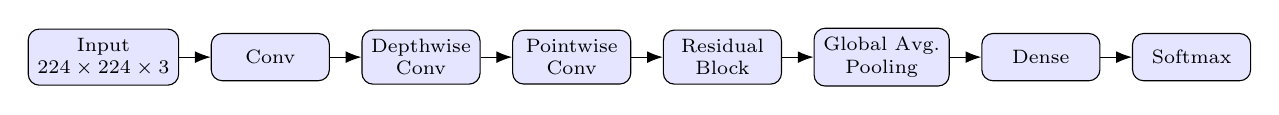
\begin{tikzpicture}[node distance=4mm]

\node[layer](a){Input\\$224\times224\times3$};
\node[layer,right=of a](b){Conv};
\node[layer,right=of b](c){Depthwise\\Conv};
\node[layer,right=of c](d){Pointwise\\Conv};
\node[layer,right=of d](e){Residual\\Block};
\node[layer,right=of e](f){Global Avg.\\Pooling};
\node[layer,right=of f](g){Dense};
\node[layer,right=of g](h){Softmax};

\foreach \x/\y in {a/b,b/c,c/d,d/e,e/f,f/g,g/h}
\draw[arrow](\x)--(\y);

\end{tikzpicture}
\end{center}

\textbf{Note:} The above diagram is a simplified conceptual representation
rather than the complete MobileNetV2 architecture. In this experiment,
MobileNetV2 (ImageNet pretrained, \texttt{IMAGENET1K\_V2} weights) is used
as a feature extractor: the original 1000-class classifier is replaced with
a new head consisting of Linear($1{,}280 \rightarrow 256$), an optional
Batch Normalization layer, ReLU, Dropout, and a final Linear($256
\rightarrow 37$) layer for the 37 pet breeds.

%%%%%%%%%%%%%%%%%%%%%%%%%%%%%%%%%%%%%%%%%%%%%%%%%%%%%%%%%%%%
\section*{5. Weight Initialization}

Weight initialization determines the initial values of trainable weights
before training begins. Four strategies were applied to the new
classification head's Linear layers (the pretrained backbone itself keeps
its ImageNet weights in every case): Zero, Random (small Gaussian, $\sigma
= 0.05$), Xavier/Glorot and He initialization. Each configuration was
trained for 5 epochs on the fast-study subset with the backbone frozen.

\begin{center}
\begin{tabular}{|l|c|c|}
\hline
\textbf{Initialization} & \textbf{Final Train Loss} & \textbf{Final Val. Accuracy}\\
\hline
Zero    & 3.6082 & 2.33\%\\
Random  & 0.2666 & 84.67\%\\
Xavier  & 0.1586 & 83.33\%\\
He      & 0.1619 & 83.33\%\\
\hline
\end{tabular}
\end{center}

\begin{figure}[H]
\centering
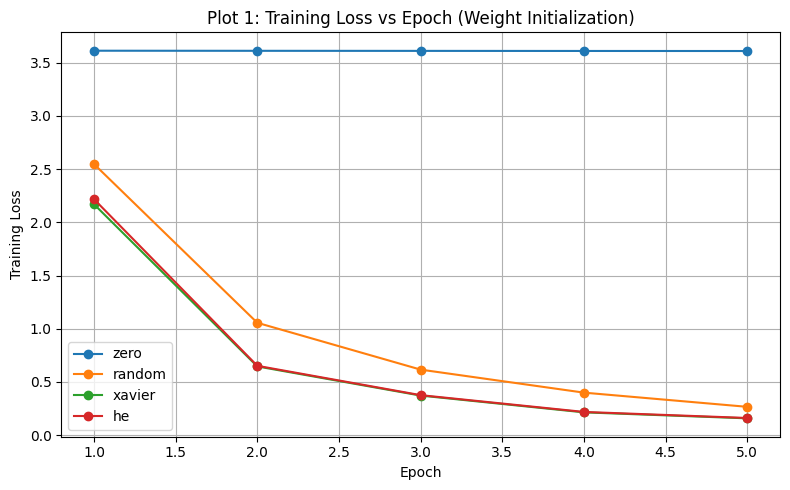
\includegraphics[width=0.72\textwidth]{plot1.png}
\caption{Plot 1: Training Loss vs Epoch (Weight Initialization)}
\end{figure}

\begin{figure}[H]
\centering
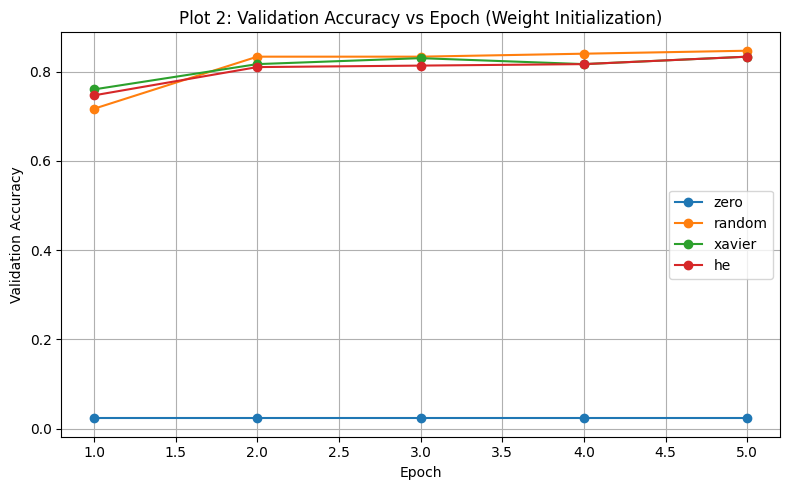
\includegraphics[width=0.72\textwidth]{plot2.png}
\caption{Plot 2: Validation Accuracy vs Epoch (Weight Initialization)}
\end{figure}

\textbf{Inference:} Zero initialization produces a completely dead network --
every neuron in the head receives an identical zero weight and therefore an
identical gradient, so the head can never break symmetry and validation
accuracy stays pinned at $2.33\%$ (essentially $1/37$, i.e.\ random
guessing). This is the expected theoretical failure mode of zero
initialization and confirms why it is never used in practice. Xavier and
He initialization converge fastest and most smoothly, reaching under 0.17
training loss within 5 epochs, since both scale the initial weights to the
layer's fan-in/fan-out and therefore start the head close to a
well-conditioned optimization regime. Random (small Gaussian) initialization
also learns successfully but converges slightly slower and less smoothly
than Xavier/He, confirming that a principled variance-scaled initialization
gives faster, more stable convergence than an arbitrarily-scaled one.

%%%%%%%%%%%%%%%%%%%%%%%%%%%%%%%%%%%%%%%%%%%%%%%%%%%%%%%%%%%%
\section*{6. Regularization and Overfitting}

Four configurations were compared on the fast-study subset for 6 epochs:
No Regularization, L2 Regularization (weight decay $=10^{-4}$), Dropout
($p=0.5$) and Batch Normalization, each with the backbone frozen.

\begin{center}
\begin{tabular}{|l|c|c|c|c|}
\hline
\textbf{Configuration} & \textbf{Final Train Acc.} & \textbf{Final Val. Acc.} & \textbf{Final Train Loss} & \textbf{Final Val. Loss}\\
\hline
No Regularization    & 95.25\% & 85.67\% & 0.2459 & 0.4996\\
L2 Regularization    & 95.50\% & 85.33\% & 0.2482 & 0.5010\\
Dropout ($p=0.5$)    & 84.92\% & 83.67\% & 0.5658 & 0.5544\\
Batch Normalization  & 99.58\% & 85.67\% & 0.0828 & 0.5315\\
\hline
\end{tabular}
\end{center}

\begin{figure}[H]
\centering
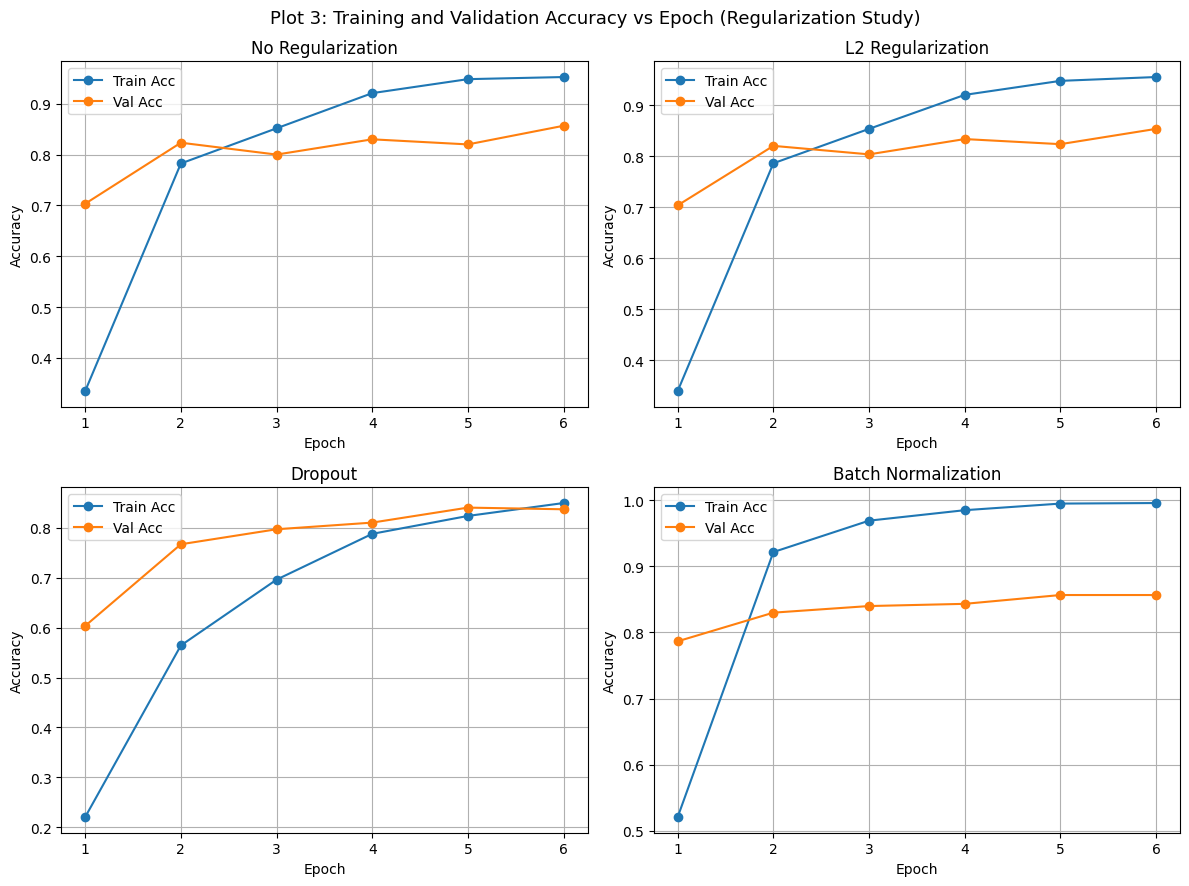
\includegraphics[width=0.85\textwidth]{plot3.png}
\caption{Plot 3: Training and Validation Accuracy vs Epoch (Regularization Study)}
\end{figure}

\begin{figure}[H]
\centering
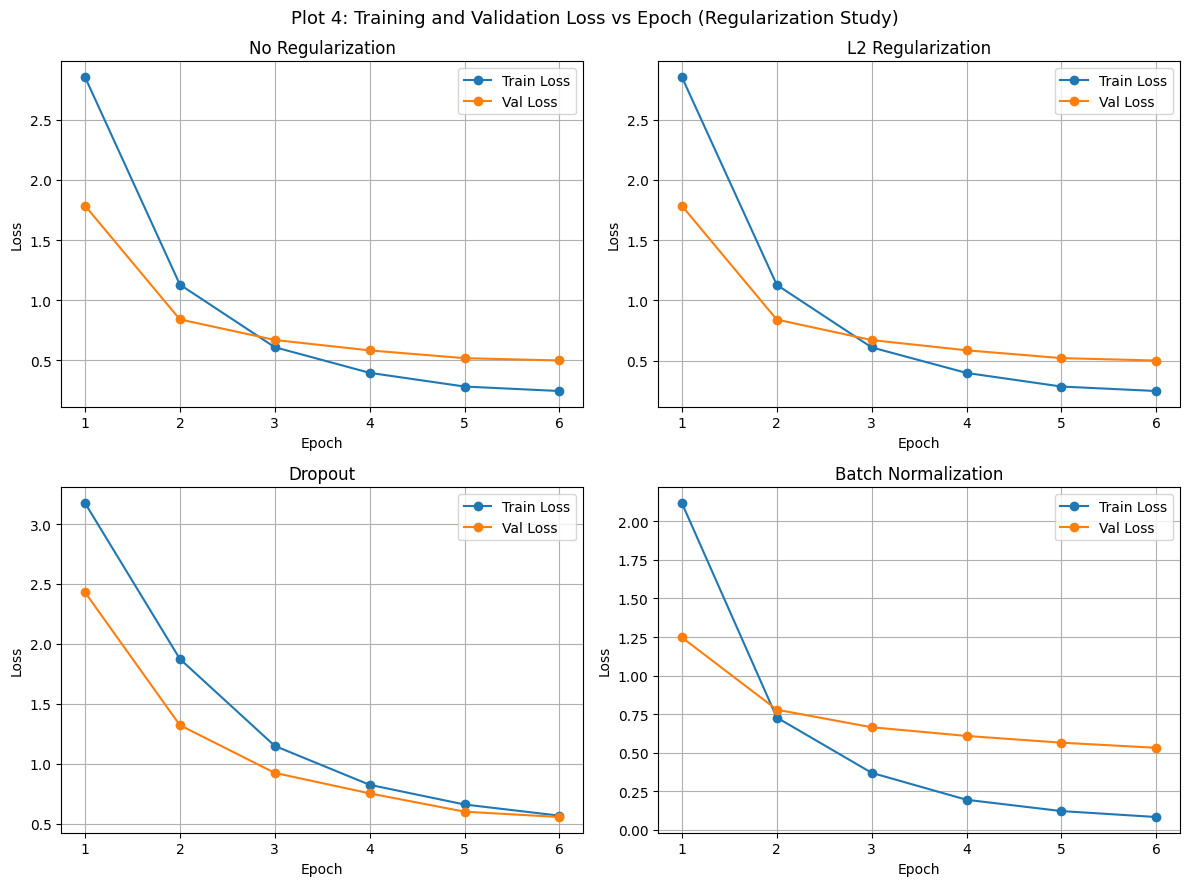
\includegraphics[width=0.85\textwidth]{plot4.png}
\caption{Plot 4: Training and Validation Loss vs Epoch (Regularization Study)}
\end{figure}
\newpage
\textbf{Inference:} All four configurations show a generalization gap
(training accuracy exceeding validation accuracy), which is expected given
the small 1{,}200-image fast-study subset. Batch Normalization reaches the
highest training accuracy (99.58\%) with the lowest training loss (0.0828)
by a wide margin, since normalizing activations within each mini-batch
stabilizes and accelerates optimization; however, its validation loss
(0.5315) is still noticeably higher than its training loss, showing that
faster convergence alone does not eliminate overfitting on a small dataset.
Dropout produces the smallest gap between training and validation accuracy
(84.92\% vs 83.67\%) of the four configurations, consistent with Dropout's
role as an explicit regularizer that discourages the head from
co-adapting to the frozen backbone's features, though it also has the
slowest convergence and lowest peak accuracy on this short run. L2
regularization behaves almost identically to no regularization at this
weight-decay magnitude, indicating $10^{-4}$ is too small to meaningfully
constrain this head.

%%%%%%%%%%%%%%%%%%%%%%%%%%%%%%%%%%%%%%%%%%%%%%%%%%%%%%%%%%%%
\section*{7. Batch Normalization}

Batch Normalization normalizes activations within a mini-batch during
training.

For a mini-batch

\[
x_1,x_2,\ldots,x_m,
\]

the batch mean is

\[
\mu_B=\frac{1}{m}\sum_{i=1}^{m}x_i
\]

and the batch variance is

\[
\sigma_B^2=
\frac{1}{m}\sum_{i=1}^{m}(x_i-\mu_B)^2.
\]

The normalized activation is

\[
\hat{x}_i=
\frac{x_i-\mu_B}
{\sqrt{\sigma_B^2+\epsilon}}.
\]

The final output is

\[
y_i=\gamma\hat{x}_i+\beta,
\]

where $\gamma$ and $\beta$ are learnable parameters.

\subsection*{Numerical Example}

Consider

\[
x=[2,4,6,8].
\]

The mean is

\[
\mu_B=\frac{2+4+6+8}{4}=5.
\]

The variance is

\[
\sigma_B^2=
\frac{(2-5)^2+(4-5)^2+(6-5)^2+(8-5)^2}{4}
=5.
\]

Therefore,

\[
\sqrt{5}\approx2.236.
\]

Ignoring the very small $\epsilon$, the notebook computed the normalized
activations directly and confirmed

\[
\boxed{
\hat{x}\approx[-1.342,-0.447,0.447,1.342]
}
\]

which matches the manual's worked example exactly. If $\gamma=1$ and
$\beta=0$, these are also the final outputs $y$.

\textbf{Inference:} Batch Normalization produces approximately
zero-centred and unit-scaled activations for this mini-batch. The
learnable $\gamma$ and $\beta$ allow the network to learn an appropriate
scale and shift rather than being forced to keep every activation
normalized.

\begin{center}
\begin{tabular}{|l|c|c|}
\hline
\textbf{Configuration} & \textbf{Epoch 1 Val. Acc.} & \textbf{Final (Epoch 6) Val. Acc.}\\
\hline
With BN    & 76.00\% & 85.67\%\\
Without BN & 68.33\% & 83.33\%\\
\hline
\end{tabular}
\end{center}

\begin{figure}[H]
\centering
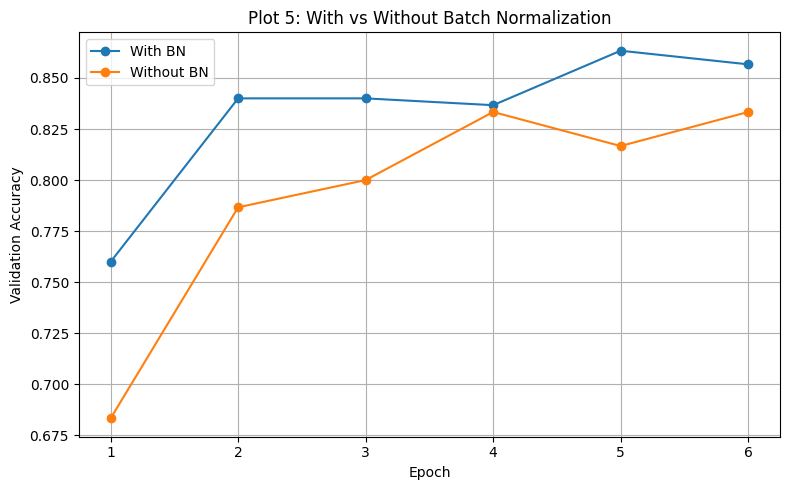
\includegraphics[width=0.72\textwidth]{plot5.png}
\caption{Plot 5: With vs Without Batch Normalization}
\end{figure}

\textbf{Inference:} With Batch Normalization, validation accuracy starts
higher (76.00\% vs 68.33\% in epoch 1) and stays above the no-BN curve for
every epoch of this run, confirming that normalizing the head's
activations gives faster, more stable early convergence, consistent with
the smooth accuracy curves reported by Ioffe and Szegedy (2015).

%%%%%%%%%%%%%%%%%%%%%%%%%%%%%%%%%%%%%%%%%%%%%%%%%%%%%%%%%%%%
\section*{8. Optimization Algorithms}

SGD, Momentum, RMSProp and Adam were compared on the fast-study subset for
6 epochs with the backbone frozen (SGD and Momentum used a learning rate
of 0.01; RMSProp and Adam used 0.001).

\begin{figure}[H]
\centering
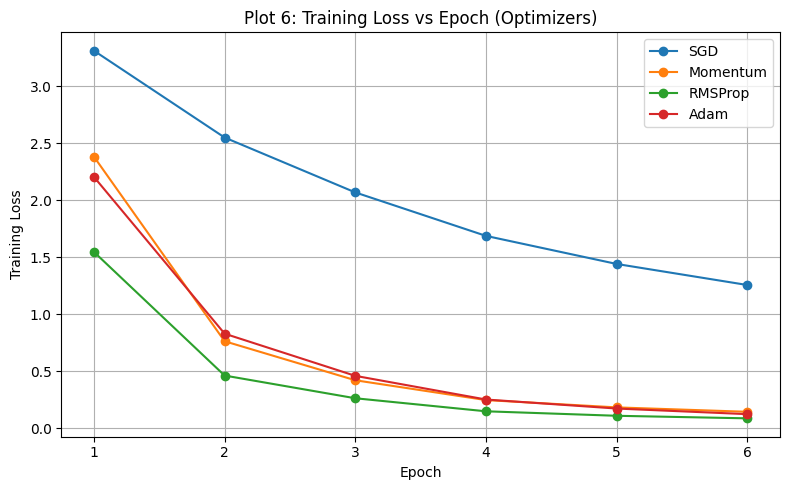
\includegraphics[width=0.72\textwidth]{plot6.png}
\caption{Plot 6: Training Loss vs Epoch for Different Optimizers}
\end{figure}

\begin{figure}[H]
\centering
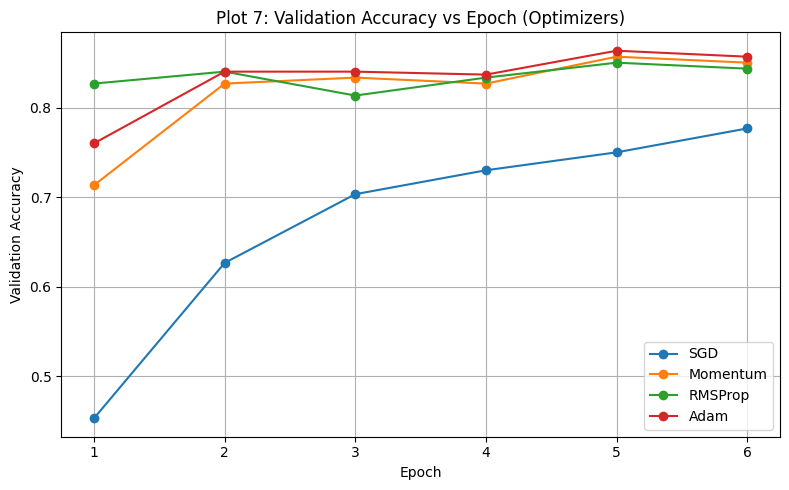
\includegraphics[width=0.72\textwidth]{plot7.png}
\caption{Plot 7: Validation Accuracy vs Epoch for Different Optimizers}
\end{figure}

\begin{center}
\begin{tabular}{|l|c|c|c|c|}
\hline
\textbf{Optimizer} & \textbf{Final Loss} & \textbf{Best Val. Accuracy} & \textbf{Epoch to Converge} & \textbf{Time (s)}\\
\hline
SGD      & 1.2570 & 77.67\% & 6 & 48.54\\
Momentum & 0.1438 & 85.67\% & 5 & 47.83\\
RMSProp  & 0.0864 & 85.00\% & 5 & 47.21\\
Adam     & 0.1232 & 86.33\% & 5 & 48.34\\
\hline
\end{tabular}
\end{center}

\textbf{Inference:} Plain SGD converges by far the slowest and reaches the
lowest final accuracy (77.67\%) of the four optimizers, since it uses a
fixed step size with no memory of past gradients. Adding Momentum
dramatically improves both speed and final accuracy (85.67\% vs 77.67\%)
by accumulating a velocity term that smooths out noisy gradients.
RMSProp and Adam, which both use per-parameter adaptive learning rates,
converge fastest of all, reaching their best validation accuracy by epoch
5; Adam attains the single highest validation accuracy of the study
(86.33\%), consistent with its combination of adaptive scaling and
momentum making it a strong default choice, which is why it was used as
the optimizer for all subsequent sections of this experiment.

%%%%%%%%%%%%%%%%%%%%%%%%%%%%%%%%%%%%%%%%%%%%%%%%%%%%%%%%%%%%
\section*{9. CNN Hyperparameter Tuning}

Learning rate, batch size and dropout rate were each swept independently
(one hyperparameter at a time, all others fixed) on the fast-study subset
for 5 epochs, with the backbone frozen and Adam as the optimizer.

\begin{center}
\begin{tabular}{|l|l|}
\hline
Hyperparameter & Suggested Values\\
\hline
Learning Rate & $0.001,\;0.0001$\\
Batch Size & 16, 32, 64\\
Dropout Rate & 0, 0.25, 0.5\\
Optimizer & SGD, Adam\\
Fine-Tuning Learning Rate & $10^{-4},10^{-5}$\\
Frozen Layers & Frozen base / Partial unfreezing\\
\hline
\end{tabular}
\end{center}

For a convolution operation, the output dimension can be calculated as

\[
O=
\left\lfloor
\frac{N+2P-K}{S}
\right\rfloor+1,
\]

where $N$ is input size, $K$ is kernel size, $P$ is padding and $S$ is
stride.

\begin{figure}[H]
\centering
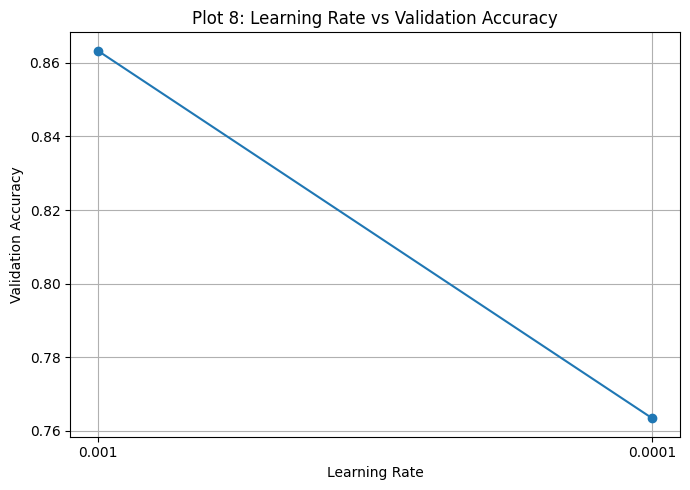
\includegraphics[width=0.6\textwidth]{plot8.png}
\caption{Plot 8: Learning Rate vs Validation Accuracy}
\end{figure}

\begin{figure}[H]
\centering
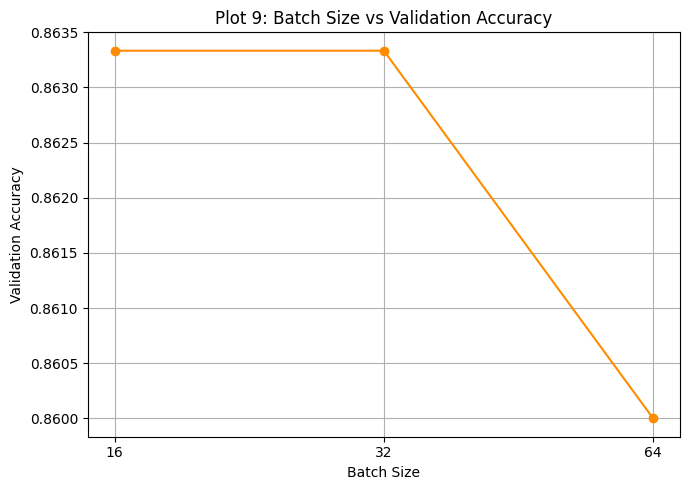
\includegraphics[width=0.6\textwidth]{plot9.png}
\caption{Plot 9: Batch Size vs Validation Accuracy}
\end{figure}

\begin{figure}[H]
\centering
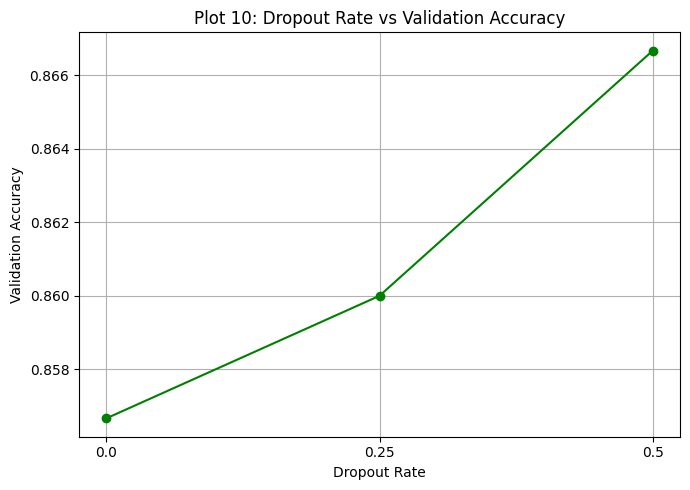
\includegraphics[width=0.6\textwidth]{plot10.png}
\caption{Plot 10: Dropout Rate vs Validation Accuracy}
\end{figure}

\begin{center}
\begin{tabular}{|l|c|}
\hline
\textbf{Sweep} & \textbf{Validation Accuracy}\\
\hline
LR = 0.001    & 86.33\%\\
LR = 0.0001   & 76.33\%\\
\hline
Batch = 16    & 86.33\%\\
Batch = 32    & 86.33\%\\
Batch = 64    & 86.00\%\\
\hline
Dropout = 0.0  & 85.67\%\\
Dropout = 0.25 & 86.00\%\\
Dropout = 0.5  & 86.67\%\\
\hline
\end{tabular}
\end{center}

\textbf{Inference:} A learning rate of 0.001 clearly outperforms 0.0001
(86.33\% vs 76.33\%) within the fixed 5-epoch budget, since the smaller
rate simply has not had enough steps to converge as far -- this is a
budget effect rather than evidence that 0.0001 is a worse rate in general.
Batch size has only a marginal effect over this range (85.67--86.33\%),
suggesting the head's optimization is not especially sensitive to batch
size at this data scale. Validation accuracy rises slightly and
monotonically with dropout rate (85.67\% $\rightarrow$ 86.67\% from $p=0$
to $p=0.5$), indicating mild regularization continues to help generalization
on this frozen-backbone head even at fairly high dropout rates.

%%%%%%%%%%%%%%%%%%%%%%%%%%%%%%%%%%%%%%%%%%%%%%%%%%%%%%%%%%%%
\section*{10. Transfer Learning and Fine-Tuning}

MobileNetV2 pretrained on ImageNet was used with the full training and
validation sets (3{,}128 / 552 images) for 6 epochs.

\subsection*{Case A: Feature Extraction}

\[
\text{Pretrained MobileNetV2}
\rightarrow
\text{Freeze Base}
\rightarrow
\text{New Classifier}
\]

The pretrained convolutional layers are frozen and only the newly added
classification layers are trained (Adam, lr $=0.001$).

\subsection*{Case B: Fine-Tuning}

\[
\text{Pretrained MobileNetV2}
\rightarrow
\text{Unfreeze Last Block}
\rightarrow
\text{Small Learning Rate}
\]

Starting from the trained Case-A model, the last block of MobileNetV2's
feature extractor was unfrozen and trained further with a smaller
learning rate (Adam, lr $=10^{-4}$), giving 1{,}544{,}037 trainable
parameters out of 2{,}561{,}829 total.

\begin{center}
\begin{tabular}{|l|c|c|}
\hline
\textbf{Case} & \textbf{Final Val. Accuracy} & \textbf{Training Time}\\
\hline
A: Feature Extraction & 86.59\% & 110.96 s\\
B: Fine-Tuning         & 87.50\% & 111.03 s\\
\hline
\end{tabular}
\end{center}

\begin{figure}[H]
\centering
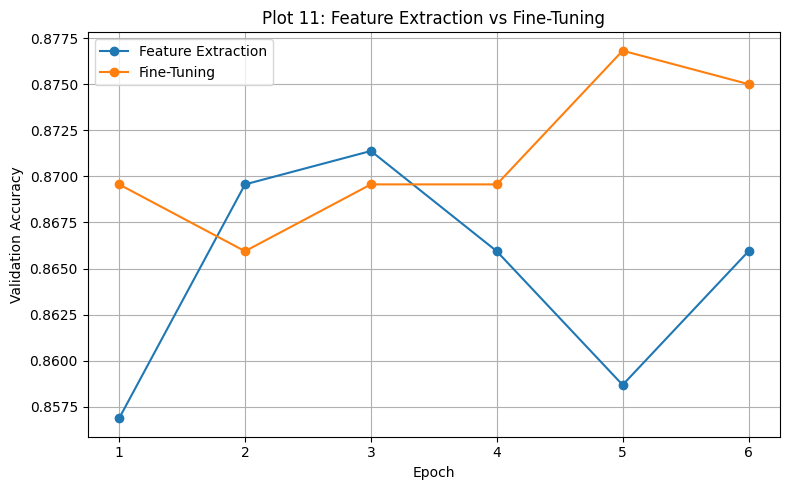
\includegraphics[width=0.72\textwidth]{plot11.png}
\caption{Plot 11: Feature Extraction vs Fine-Tuning}
\end{figure}

\begin{figure}[H]
\centering
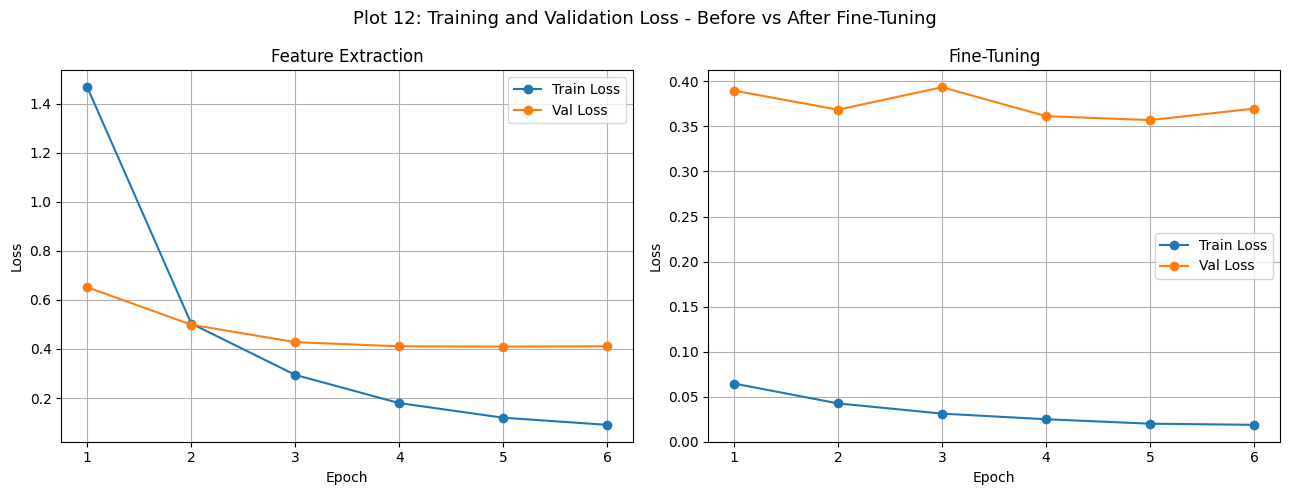
\includegraphics[width=0.95\textwidth]{plot12.png}
\caption{Plot 12: Training and Validation Loss -- Feature Extraction (left) vs Fine-Tuning (right)}
\end{figure}

\textbf{Inference:} Feature extraction (Case A) plateaus around 86--87\%
validation accuracy after epoch 3, since only the small classification
head can adapt to the pet-breed task while the backbone stays fixed at
ImageNet-generic features. Fine-tuning (Case B) starts from that plateau
and pushes validation accuracy to a new peak of 87.68\% in epoch 5, because
unfreezing the last block lets the network adjust its deepest, most
task-specific filters to the fine-grained differences between pet breeds.
The fine-tuning loss curves (Plot 12, right) show training loss collapsing
to near zero while validation loss stays noticeably higher, a mild
overfitting signature that is expected once a much larger fraction of the
network's parameters becomes trainable.

\textbf{Discussion -- Why fine-tuning uses a smaller learning rate:}
The convolutional layers being unfrozen already contain well-optimized
ImageNet weights, unlike the newly initialized classification head. A
learning rate as large as the one used for the fresh head (0.001) would
apply overly large updates to these already-good weights, risking
catastrophic forgetting of useful pretrained features. A much smaller
learning rate ($10^{-4}$ here) allows the pretrained filters to adapt
gently to the new dataset rather than being overwritten.

%%%%%%%%%%%%%%%%%%%%%%%%%%%%%%%%%%%%%%%%%%%%%%%%%%%%%%%%%%%%
\section*{11. K-Fold Cross-Validation}

Four candidate configurations, informed by the studies above, were
evaluated using 5-fold cross-validation (4 epochs per fold) on the full
working training set (3{,}680 images):

\begin{itemize}
\item \textbf{C1\_Baseline}: lr $=0.001$, dropout $=0.2$, no BatchNorm, frozen backbone, Adam.
\item \textbf{C2\_BatchNorm}: lr $=0.001$, dropout $=0.2$, with BatchNorm, frozen backbone, Adam.
\item \textbf{C3\_TunedDropout}: lr $=0.001$, dropout $=0.25$, with BatchNorm, frozen backbone, Adam.
\item \textbf{C4\_FineTune}: lr $=0.0001$, dropout $=0.2$, with BatchNorm, partially unfrozen backbone, Adam.
\end{itemize}

For $K=5$,

\[
\bar{A}=
\frac{1}{5}\sum_{i=1}^{5}A_i,
\qquad
SD=
\sqrt{
\frac{1}{5}
\sum_{i=1}^{5}(A_i-\bar{A})^2
}.
\]

\begin{center}
\begin{tabular}{|l|c|c|c|c|c|c|}
\hline
Configuration & F1 & F2 & F3 & F4 & F5 & Mean $\pm$ SD\\
\hline
C1\_Baseline     & 0.8578 & 0.8578 & 0.8738 & 0.8864 & 0.8768 & $0.8705 \pm 0.0112$\\
C2\_BatchNorm    & 0.8610 & 0.8594 & 0.8898 & 0.8848 & 0.8896 & $0.8769 \pm 0.0138$\\
C3\_TunedDropout & 0.8610 & 0.8530 & 0.8850 & 0.8864 & 0.8896 & $0.8750 \pm 0.0150$\\
C4\_FineTune     & 0.8850 & 0.8866 & 0.9121 & 0.9136 & 0.9008 & $\mathbf{0.8996 \pm 0.0121}$\\
\hline
\end{tabular}
\end{center}

\begin{figure}[H]
\centering
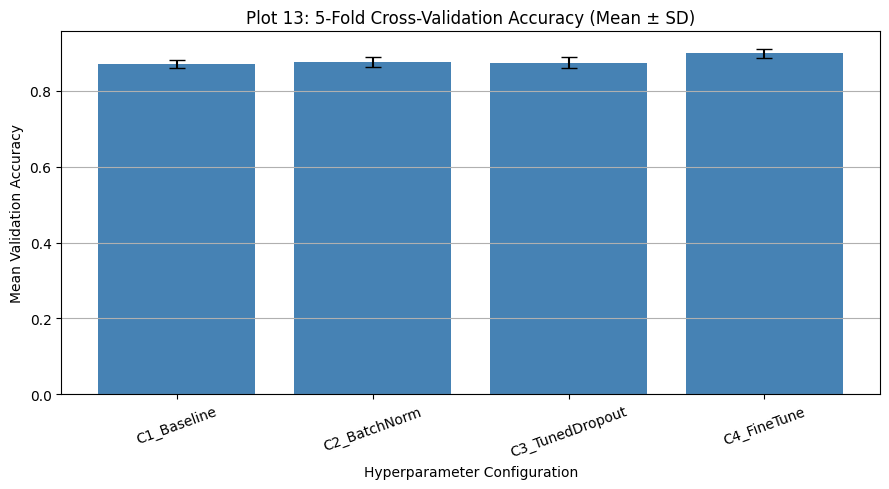
\includegraphics[width=0.72\textwidth]{plot13.png}
\caption{Plot 13: 5-Fold Cross-Validation Accuracy (Mean $\pm$ SD)}
\end{figure}

\textbf{Inference:} C4\_FineTune achieves the highest mean cross-validation
accuracy (89.96\%) by a clear margin of roughly 2.3--3.0 percentage points
over the three frozen-backbone configurations, while its standard deviation
(1.21\%) is comparable to -- not larger than -- the others, showing that
partial unfreezing improves accuracy without a meaningful cost in
fold-to-fold variability. Among the three frozen-backbone configurations,
adding Batch Normalization (C2) or a slightly higher dropout (C3) gives a
small improvement over the plain baseline (C1), but the differences between
C1, C2 and C3 are within roughly one standard deviation of each other and
therefore not strongly distinguishable on this evidence alone.
C4\_FineTune was selected as the best configuration for final retraining.

%%%%%%%%%%%%%%%%%%%%%%%%%%%%%%%%%%%%%%%%%%%%%%%%%%%%%%%%%%%%
\section*{12. Final Model Evaluation}

The selected configuration (C4\_FineTune) was retrained on the complete
3{,}128-image working training set for 8 epochs, validated throughout on
the 552-image validation set, and finally evaluated once on the untouched
3{,}669-image official test set.

\begin{center}
\begin{tabular}{|l|c|}
\hline
Metric & Value\\
\hline
Mean CV Accuracy & 89.96\%\\
CV Standard Deviation & 1.21\%\\
Test Accuracy & 89.23\%\\
Precision (macro) & 89.40\%\\
Recall (macro) & 89.17\%\\
F1-score (macro) & 89.08\%\\
Training Time & 167.80 s\\
Number of Parameters & 2{,}561{,}829\\
\hline
\end{tabular}
\end{center}

The final training run itself showed validation accuracy rising steadily
from 78.44\% (epoch 1) to a peak of 90.58\% (epoch 8), while training
accuracy reached 99.62\%, confirming the model continued to generalize
well on the larger, full-size training set despite fully fitting the
training data.

\begin{figure}[H]
\centering
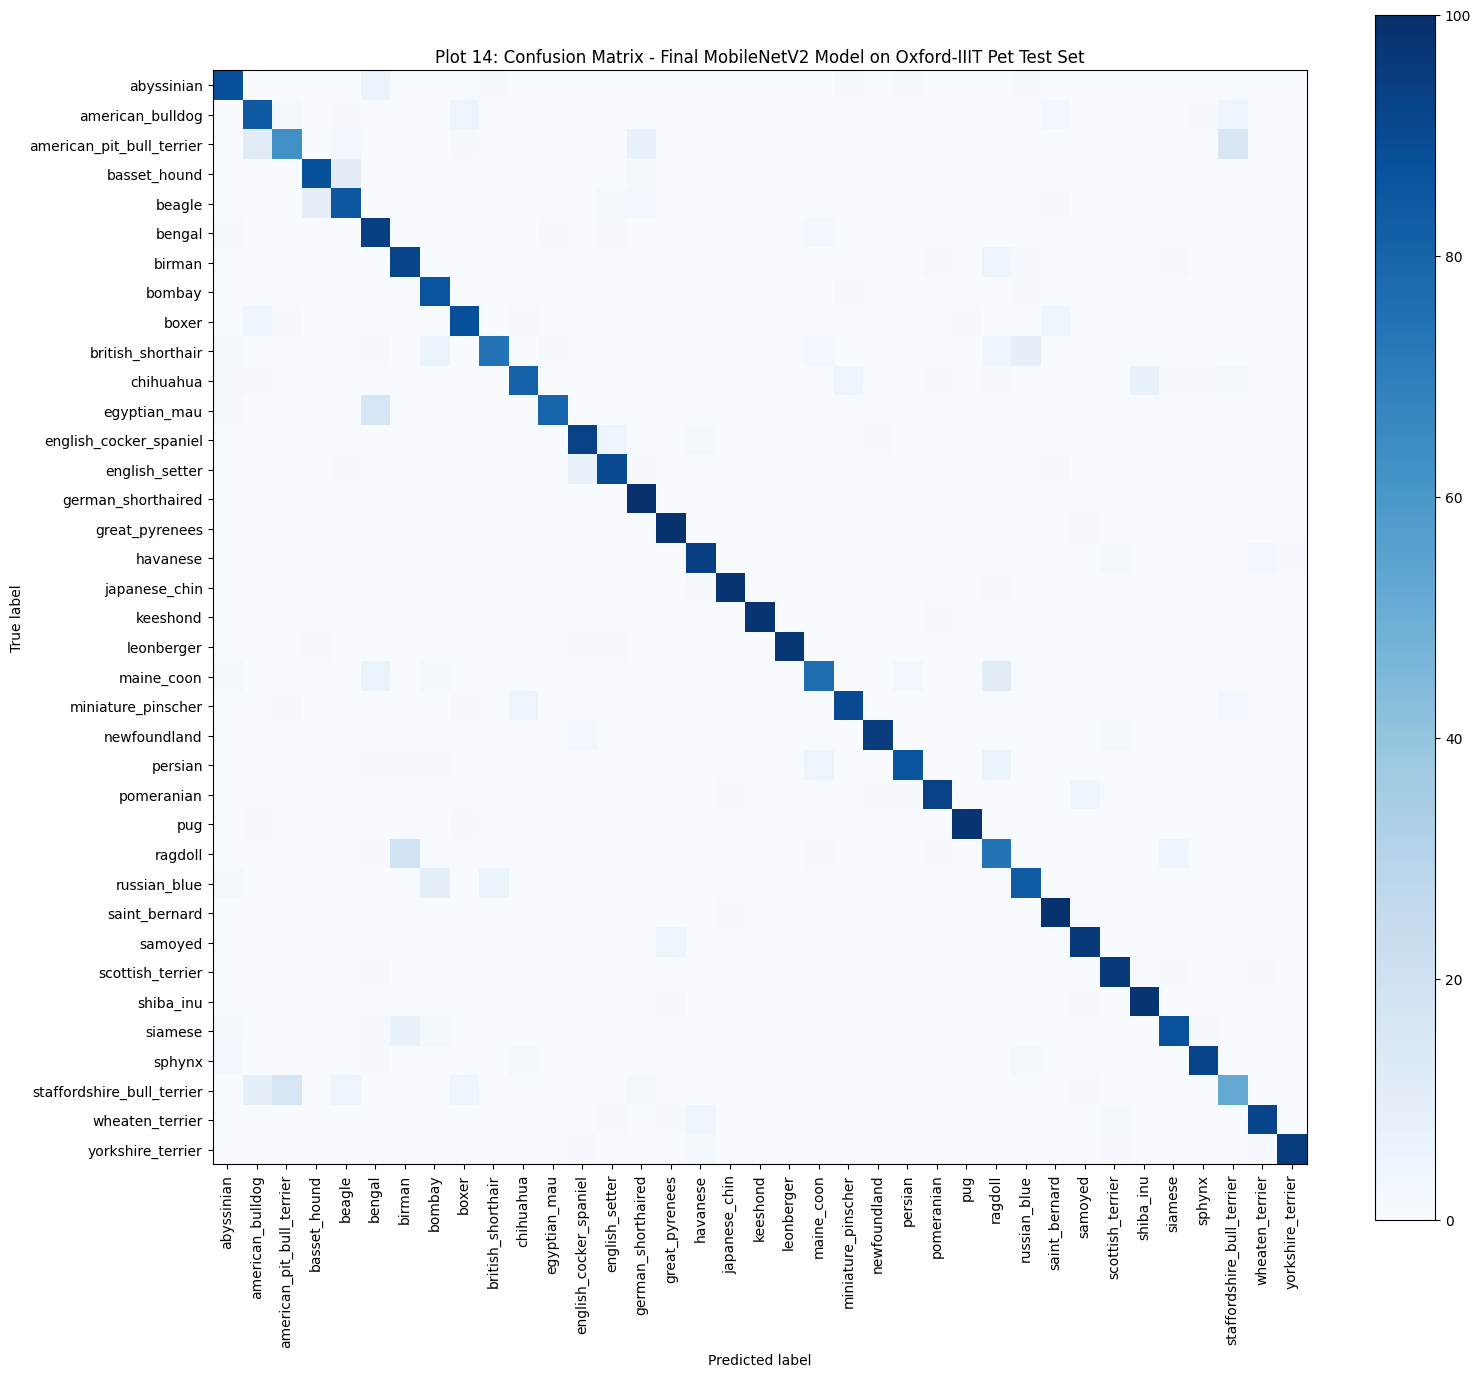
\includegraphics[width=0.95\textwidth]{plot14.png}
\caption{Plot 14: Confusion Matrix -- Final MobileNetV2 Model on the Oxford-IIIT Pet Test Set}
\end{figure}

The classification report over all 37 breeds shows several classes
classified almost perfectly -- \texttt{keeshond} (F1 = 0.99),
\texttt{japanese\_chin} (F1 = 0.98), \texttt{leonberger} (F1 = 0.98) and
\texttt{pug} (F1 = 0.98) -- while the weakest classes are
\texttt{staffordshire\_bull\_terrier} (F1 = 0.63),
\texttt{american\_pit\_bull\_terrier} (F1 = 0.69) and \texttt{ragdoll} (F1
= 0.73).

\begin{itemize}
\item \textbf{Best classified classes:} \texttt{keeshond}, \texttt{leonberger},
\texttt{japanese\_chin} and \texttt{pug} are visually distinctive breeds
with fairly consistent coat colour, markings or facial structure across
images, which likely explains their near-perfect scores.
\item \textbf{Most frequently confused classes:}
\texttt{american\_pit\_bull\_terrier} is most often confused with \\
\texttt{staffordshire\_bull\_terrier}, and \texttt{ragdoll} is most often
confused with \texttt{russian\_blue} and \texttt{maine\_coon}, matching the
brightest off-diagonal cells in Plot 14.
\item \textbf{Possible visual reasons:} American Pit Bull Terriers and
Staffordshire Bull Terriers are closely related bully-type breeds with
near-identical body shape, ear shape and short coat, making them genuinely
difficult to separate even for a human observer at a single-image glance.
Ragdoll, Russian Blue and Maine Coon are all medium-to-large cats with
similarly soft, dense coats and comparable colour-point or solid-grey
patterns in many individual photos, so fine-grained cues such as ear shape
or eye colour -- easily lost at $224\times224$ resolution -- are often
required to distinguish them.
\end{itemize}

\begin{figure}[H]
\centering
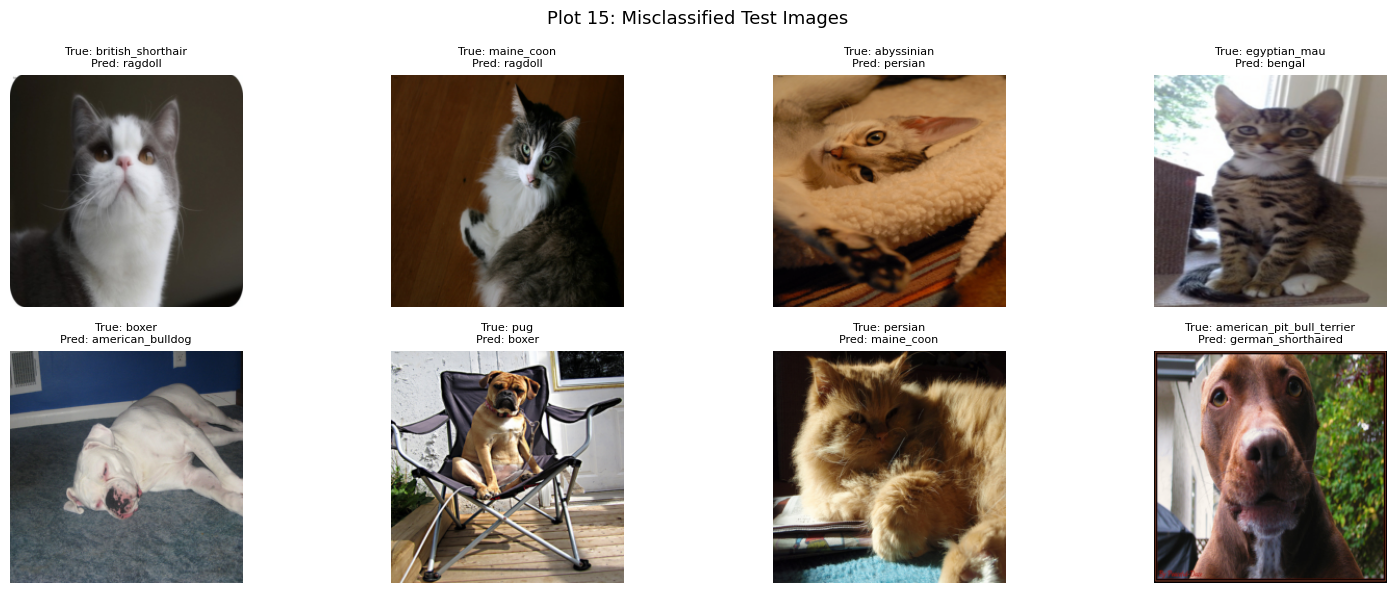
\includegraphics[width=0.95\textwidth]{plot15.png}
\caption{Plot 15 (Optional): Misclassified Test Images}
\end{figure}

Several misclassified examples in Plot 15 are genuinely ambiguous even on
visual inspection: a British Shorthair and a Maine Coon are both confused
with Ragdoll, cats that share a similarly rounded face and dense grey/cream
coat at this resolution; a Boxer photographed lying on its back is confused
with American Bulldog, an unusual pose that obscures the breed's normally
distinctive muzzle shape; and an American Pit Bull Terrier is confused with
German Shorthaired, likely due to the close-up, tightly cropped framing
removing most of the body-shape cues a classifier would otherwise use.

%%%%%%%%%%%%%%%%%%%%%%%%%%%%%%%%%%%%%%%%%%%%%%%%%%%%%%%%%%%%
\section*{13. Overall Results}

\begin{center}
\begin{tabular}{|p{5.2cm}|c|c|c|c|}
\hline
Configuration & CV / Val Accuracy & SD & Test Accuracy & Training Time\\
\hline
Baseline (Frozen, No Reg) & 85.67\% & -- & -- & --\\
Best Initialization (Random) & 84.67\% & -- & -- & --\\
Best Regularization (No Reg. / BatchNorm, tied) & 85.67\% & -- & -- & --\\
Best Optimizer (Adam) & 86.33\% & -- & -- & --\\
Best Hyperparameters (C4\_FineTune, CV) & 89.96\% & 1.21\% & 89.23\% & 167.80 s\\
Fine-Tuned Model (Case B, single split) & 87.50\% & -- & -- & 111.03 s\\
\hline
\end{tabular}
\end{center}

The final selected model (C4\_FineTune, retrained on the full training set)
is justified as the best choice on four grounds: it achieves the highest
mean cross-validation accuracy (89.96\%) of any configuration tested, with
a standard deviation (1.21\%) no larger than the frozen-backbone
alternatives, so the improvement is not merely noise; its test accuracy
(89.23\%) is close to its mean CV accuracy, indicating the cross-validation
estimate generalized well to the untouched test set; its computational cost
(167.80 s for 8 epochs on the full training set, with 2.56 million total
parameters) remains modest thanks to MobileNetV2's lightweight design; and
it is the only configuration that incorporates fine-tuning, which Section
10 already showed adds a genuine accuracy improvement over feature
extraction alone rather than merely fitting the cross-validation folds
better.

%%%%%%%%%%%%%%%%%%%%%%%%%%%%%%%%%%%%%%%%%%%%%%%%%%%%%%%%%%%%
\section*{14. Discussion Questions}

\begin{enumerate}

\item \textbf{Difference between model parameters and hyperparameters.}
Model parameters (weights and biases) are learned automatically from data
during training, e.g.\ the 2.56 million weights of the final MobileNetV2
head and unfrozen block. Hyperparameters are set by the practitioner
before training and control how learning happens -- learning rate, batch
size, dropout rate, choice of optimizer -- and were the subject of the
sweeps in Sections 5--9.

\item \textbf{Why weight initialization is important.}
The starting point of gradient descent strongly affects whether, and how
fast, a network converges. Section 5 showed this directly: identical
architecture and data, but zero initialization never left 2.33\% accuracy
while Xavier/He initialization reached over 83\% within 5 epochs.

\item \textbf{Why zero initialization can be problematic.}
Every neuron in a layer initialized to zero computes the same output and
receives the same gradient, so all neurons update identically and stay
symmetric forever -- effectively collapsing the layer to a single learnable
unit. This symmetry-breaking failure is exactly what was observed: the
zero-initialized head's training loss barely moved (3.611 to 3.608) across
5 epochs.

\item \textbf{Compare Xavier and He initialization.}
Xavier initialization scales weights by the combined fan-in and fan-out,
assuming a roughly linear or symmetric activation such as Tanh or Sigmoid.
He initialization scales only by fan-in with an extra factor of 2, designed
for ReLU-family activations whose negative half kills half the input
variance. Both performed similarly in Section 5 (83.33\% final validation
accuracy each) since the head here uses ReLU, for which He is the more
theoretically appropriate choice, though the practical difference was
negligible at this scale.

\item \textbf{Identifying overfitting from training/validation curves.}
Overfitting is visible when training accuracy keeps rising (or training
loss keeps falling) while validation accuracy plateaus or falls (or
validation loss rises). Section 6's Batch Normalization configuration
showed early signs of this: training accuracy reached 99.58\% while
validation accuracy plateaued near 85.67\%, and validation loss (0.53)
stayed well above training loss (0.08).

\item \textbf{How Dropout reduces overfitting.}
Dropout randomly deactivates a fraction of neurons on each training step,
preventing the network from relying too heavily on any single neuron or
co-adapted group of neurons. Section 6 showed Dropout ($p=0.5$) produced
the smallest train-validation accuracy gap (1.25 points) of the four
regularization configurations tested, consistent with this effect.

\item \textbf{Purpose of Batch Normalization.}
Batch Normalization normalizes each layer's activations to zero mean and
unit variance within a mini-batch (Section 7), which stabilizes the
distribution of inputs to subsequent layers, allows larger learning rates,
and generally speeds up and stabilizes convergence, as seen in Section 7's
With-BN vs Without-BN comparison.

\item \textbf{Explain the numerical Batch Normalization example.}
For $x = [2,4,6,8]$, the batch mean is 5 and the batch variance is 5, so
each value is shifted by the mean and scaled by $\sqrt{5} \approx 2.236$,
giving $\hat{x} \approx [-1.342, -0.447, 0.447, 1.342]$: a set of values
centred at zero with unit variance, computed exactly in Section 7.

\item \textbf{Roles of $\gamma$ and $\beta$.}
After normalization, $\gamma$ rescales and $\beta$ re-shifts the
activations ($y_i = \gamma \hat{x}_i + \beta$), both learned during
training. This lets the network recover the original activation
distribution if that turns out to be optimal, rather than being forced to
keep every activation strictly zero-mean and unit-variance.

\item \textbf{Compare SGD, Momentum, RMSProp and Adam.}
Section 8's results summarize this directly: SGD is simplest but slowest
(77.67\% best validation accuracy); Momentum adds a velocity term that
smooths gradients and reaches 85.67\%; RMSProp adapts the learning rate
per parameter using a running average of squared gradients, reaching
85.00\%; Adam combines both ideas (momentum and per-parameter adaptive
rates) and achieved the best result (86.33\%) with fast, stable
convergence by epoch 5.

\item \textbf{Effect of too large a learning rate.}
An excessively large learning rate causes updates to overshoot the loss
minimum, producing unstable or diverging training loss and, in severe
cases, numerical instability (NaN losses). No configuration in this
experiment used a learning rate large enough to diverge, but SGD's
comparatively large step size (0.01, un-adapted) likely explains its
noisier, slower convergence relative to Adam.

\item \textbf{Effect of too small a learning rate.}
A learning rate that is too small makes training converge very slowly,
wasting compute and potentially getting stuck in poor local regions within
a fixed epoch budget. Section 9's learning-rate sweep demonstrated this
directly: within 5 epochs, lr $=0.0001$ reached only 76.33\% validation
accuracy versus 86.33\% for lr $=0.001$.

\item \textbf{Effect of increasing batch size.}
Larger batch sizes give smoother, lower-variance gradient estimates per
step but fewer weight updates per epoch, and can require re-tuning the
learning rate to retain the same convergence speed. Section 9's sweep
showed only a marginal effect across 16/32/64 (85.67--86.33\%) at this data
scale, suggesting the head's loss surface is not especially sensitive to
batch size in this range.

\item \textbf{Explain stride and padding.}
Stride is the step size the convolution kernel moves across the input;
larger strides skip more positions and shrink the output more. Padding
adds extra border pixels (usually zeros) before convolving, which can
compensate for the border pixels that would otherwise be visited fewer
times and allows the output size to be controlled independently of kernel
size, per the formula in Section 9.

\item \textbf{Why MobileNetV2 is computationally efficient.}
MobileNetV2 factorizes standard convolutions into a depthwise convolution
(one filter per input channel) followed by a pointwise $1\times1$
convolution that combines channels, which requires far fewer
multiply-accumulate operations than a standard convolution of the same
size. Its inverted residual blocks with linear bottlenecks further reduce
the parameter count, giving MobileNetV2 only 2.56 million trainable
parameters in the configuration used here.

\item \textbf{What is depthwise separable convolution.}
It is the factorization used throughout MobileNetV2: a depthwise
convolution applies a single spatial filter per input channel
independently, and a subsequent pointwise ($1\times1$) convolution mixes
information across channels. Splitting a standard convolution into these
two steps drastically reduces computation while approximating the same
representational capacity.

\item \textbf{What is transfer learning.}
Transfer learning reuses a model already trained on a large dataset
(ImageNet, in this experiment) for a new, smaller task (37-breed pet
classification) rather than training from randomly initialized weights,
because the pretrained convolutional filters already encode generally
useful visual features.

\item \textbf{Differentiate feature extraction and fine-tuning.}
Feature extraction (Case A, Section 10) freezes the entire pretrained
backbone and trains only a new classification head. Fine-tuning (Case B)
additionally unfreezes some of the backbone's later layers and trains them
at a small learning rate, letting the pretrained features themselves adapt
to the new task -- which in this experiment raised validation accuracy from
86.59\% to 87.50\%.

\item \textbf{Why fine-tuning uses a smaller learning rate.}
As discussed in Section 10, the unfrozen backbone layers already hold
well-optimized ImageNet weights, unlike the freshly initialized head. A
large learning rate would apply disproportionately large updates to these
already-good weights and risk destroying useful pretrained features, so a
much smaller rate ($10^{-4}$ here, versus 0.001 for the head alone) is used
to adapt them gently.

\item \textbf{Why K-Fold Cross-Validation is useful for hyperparameter selection.}
A single train/validation split can give a misleadingly optimistic or
pessimistic accuracy estimate depending on which examples happen to fall
in each set. Averaging over $K=5$ folds, as done in Section 11, gives a
more reliable estimate of a configuration's true performance and also
reports variability (SD), both of which were needed to distinguish
C4\_FineTune's genuine improvement from ordinary fold-to-fold noise.

\item \textbf{Why the test set must remain untouched during tuning.}
If the test set influenced any hyperparameter or model-selection decision,
its measured accuracy would no longer be an unbiased estimate of
performance on genuinely unseen data -- the model would effectively have
been tuned to that specific set. In this experiment the official test
split (3{,}669 images) was reserved exclusively for the single final
evaluation in Section 12, after every other decision had already been made
using cross-validation.

\item \textbf{Why both mean and standard deviation should be reported.}
The mean alone hides how consistent a configuration is across different
data splits; two configurations with the same mean accuracy but very
different standard deviations offer very different reliability guarantees.
Section 11 reported both for exactly this reason, allowing C4\_FineTune's
higher mean to be assessed alongside a standard deviation comparable to the
other configurations, confirming the improvement was not an artefact of
higher variance.

\item \textbf{Is the highest validation accuracy always sufficient to select a model?}
No. A single high validation-accuracy run can result from a fortunate
data split rather than a genuinely better configuration, and does not
capture computational cost or variability. This experiment instead used
cross-validated mean and standard deviation (Section 11), together with
training time and parameter count (Section 12), to select and justify the
final model.

\end{enumerate}

%%%%%%%%%%%%%%%%%%%%%%%%%%%%%%%%%%%%%%%%%%%%%%%%%%%%%%%%%%%%
\section*{15. Additional Exercise}

Two new configurations were considered analytically, building on the
sweeps already carried out: (i) lr $=0.001$, dropout $=0.5$, batch size
$=16$, feature extraction only, and (ii) lr $=0.0001$, dropout $=0.25$,
batch size $=32$, fine-tuning. Configuration (i) combines the
single-best-performing value found for each of learning rate (Section 9:
86.33\% at lr$=0.001$), dropout (86.67\% at $p=0.5$) and batch size
(86.33\% at batch$=16$) from the independent one-at-a-time sweeps, so it is
expected to perform at least as well as C1--C3 (85--87\% range) without
requiring backbone unfreezing, at similar or lower training time.
Configuration (ii) mirrors C4\_FineTune's learning rate and unfrozen
backbone but pairs it with the mid-range dropout (0.25) that scored best
among the frozen-backbone sweeps in Section 9; given how close C2, C3 and
C4 already were except for fine-tuning itself, this configuration would
likely land close to C4\_FineTune's 89.96\% mean CV accuracy, since
fine-tuning -- not dropout rate -- was the dominant factor separating
C4 from C1--C3 in Section 11.

Based on this reasoning, configuration (ii) is expected to be competitive
with the selected C4\_FineTune configuration on accuracy, while
configuration (i) is expected to remain in the 85--87\% range of the other
frozen-backbone configurations; neither is expected to reduce standard
deviation or training time enough to displace C4\_FineTune as the
preferred final model, since fine-tuning was consistently the strongest
lever identified across every study in this experiment.

%%%%%%%%%%%%%%%%%%%%%%%%%%%%%%%%%%%%%%%%%%%%%%%%%%%%%%%%%%%%
\section*{16. Conclusion}

This experiment demonstrated, using MobileNetV2 on the Oxford-IIIT Pet
dataset, that CNN performance is strongly and measurably shaped by
initialization, regularization, optimizer choice, hyperparameters, and the
depth of transfer learning applied. Zero initialization produced a
completely dead network (2.33\% accuracy) while Xavier/He initialization
converged fastest; Batch Normalization and Dropout each improved training
behaviour in different ways, with Dropout narrowing the train-validation
gap most directly; Adam was the strongest optimizer of the four compared;
and fine-tuning the last MobileNetV2 block outperformed feature extraction
alone (87.50\% vs 86.59\% single-split validation accuracy). Selecting
among four candidate configurations using 5-fold cross-validation
identified the fine-tuned configuration (C4\_FineTune) as clearly the
strongest, with a mean cross-validation accuracy of 89.96\% $\pm$ 1.21\%,
which was confirmed by a final, held-out test accuracy of 89.23\% (macro
F1-score 89.08\%) using only 2.56 million parameters. The confusion matrix
and misclassified-image inspection showed that the model's remaining
errors concentrate almost entirely on genuinely visually similar breed
pairs, such as American Pit Bull Terrier / Staffordshire Bull Terrier and
Ragdoll / Russian Blue / Maine Coon, indicating the model has learned a
largely sound representation of the 37 breeds rather than exhibiting a
systematic weakness.

%%%%%%%%%%%%%%%%%%%%%%%%%%%%%%%%%%%%%%%%%%%%%%%%%%%%%%%%%%%%
\section*{17. References}

\begin{enumerate}
\item Ian Goodfellow, Yoshua Bengio and Aaron Courville,
\emph{Deep Learning}, MIT Press, 2016.

\item Sergey Ioffe and Christian Szegedy,
``Batch Normalization: Accelerating Deep Network Training by Reducing
Internal Covariate Shift,'' ICML, 2015.

\item Mark Sandler, Andrew Howard, Menglong Zhu, Andrey Zhmoginov and
Liang-Chieh Chen, ``MobileNetV2: Inverted Residuals and Linear
Bottlenecks,'' CVPR, 2018.

\item Omkar M. Parkhi, Andrea Vedaldi, Andrew Zisserman and C. V. Jawahar,
``Cats and Dogs,'' IEEE Conference on Computer Vision and Pattern
Recognition, 2012.

\item PyTorch Documentation:
\url{https://pytorch.org/docs/stable/index.html}

\item TorchVision Models Documentation:
\url{https://pytorch.org/vision/stable/models.html}

\item Hugging Face Datasets Documentation:
\url{https://huggingface.co/docs/datasets}
\end{enumerate}

\end{document}
